\graphicspath{{./figures}}

\section{Tracking}

\subsection{Open-Loop}

In order to test the GPS pointing and open-loop tracking, a map was printed with lines pointing to locations in the area from a pre-determined location. The ground station was then placed on top of the map at this location, and positioned to face magnetic north using a compass. This test had multiple goals: the mount transfer function, the GPS co-ordinate pointing, and the flight path data following, were all tested simultaneously. An image of the test setup is shown in Figure \ref{fig:pointingTest}.

\begin{figure}[!htb]
  \centering
  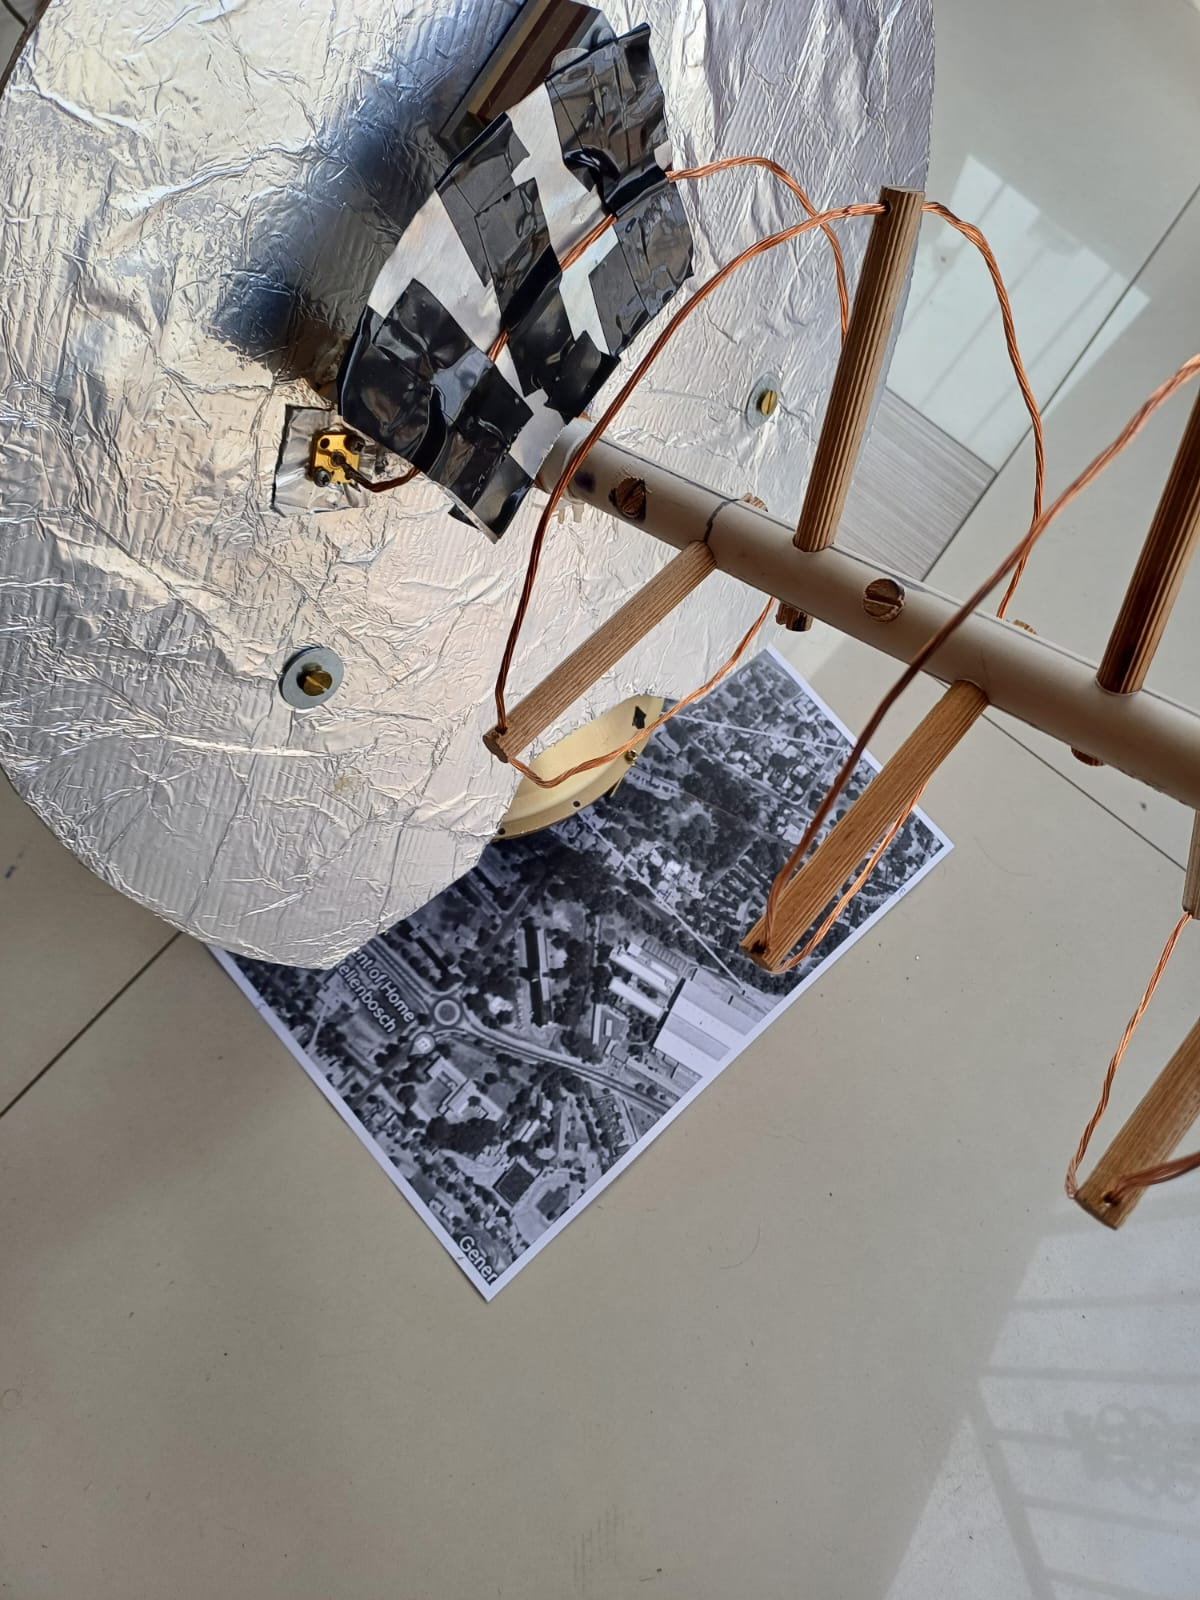
\includegraphics[width=0.4\textwidth]{pointingTestSetup}
  \caption{Pointing Test Setup}
  \label{fig:pointingTest}
\end{figure}

Flight path data containing the pre-determined co-ordinates was then uploaded to the system, and the azimuthal angle was qualitatively confirmed to point in the directions labeled on the map. Further, the elevation angle was measured using a protractor and compared against the expected angle. The system was found to successfully point towards the commanded locations at the desired times. The elevation angle measured were found to be within $5^\circ$ of the expected angle. This is considered to be within the limitations of the measurements, as the setup to measure the incline of the ground plane was non-ideal.

\subsection{Closed-Loop}

The closed-loop recieved location GPS tracking was tested on an open field at aroudn 300 m range. The PQ unit was carried around the field transmitting its GPS location, and the RSSI was recorded, as well as the pointing direction qualitatively noted.

\begin{figure}[!htb]
  \centering
  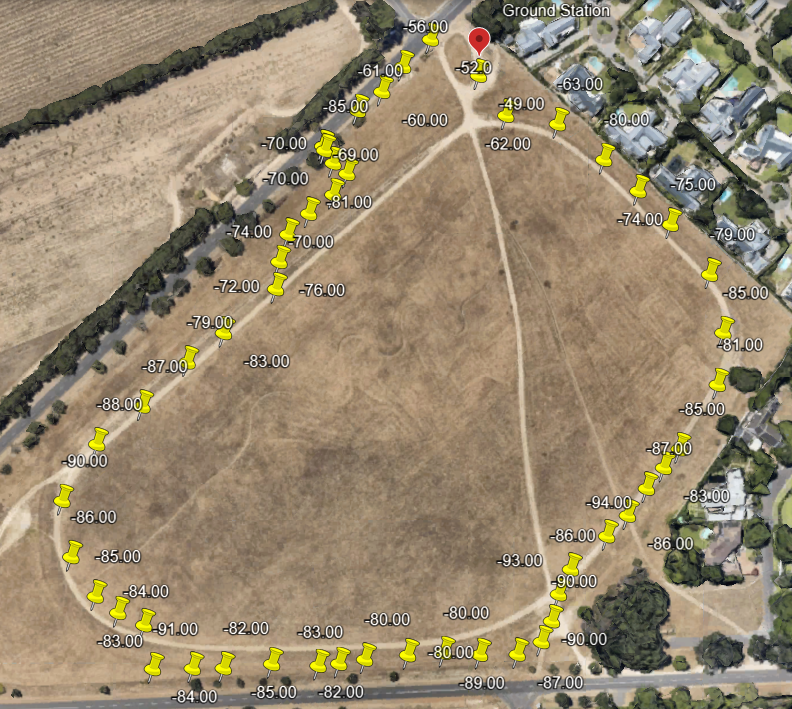
\includegraphics[width=0.7\textwidth]{gpsTrackingMap}
  \caption{GPS Tracking Locations and RSSI Values}
  \label{fig:gpsTrackingMap}
\end{figure}

The system was observed to successfully track the transmitter around the entire field without noticeable delay, until it reached a distance of around 10 m, where the pointing direction became unpredictable. This is attributed to the low accuracy of the GPS modules. Since the system is already known to have the capabilities of pointing at a GPS location (from the open-loop tests) and the time requirement is much lower for the balloon satellite system (which requires a tracking speed on the order of 45 degrees in an hour or two) it is clear the system works as designed.

The above test also acts as a primitive test for GPS accuracy, however. The width of the main path being walked on was 3.2 m wide. The furthest deviation of a received GPS co-ordinate from this path is around 3 m (note that the map image is outdated). Therefore, an upper bound on the GPS's accuracy can be set at 6.2 m. Since the required accuracy for the system was calculated to be on the order of a thousand metres (though low is preferable) this setup is deemed to be acceptable.